\chapter{Results}\label{cha:results}
\todo[inline]{Att lägga till: Execution time för planeraren, robusthet under varierande vind, förhoppningsvis flygningar med riktig drönare}
The proposed framework was evaluated by performing a number of simulations in the ArduPlane SITL environment, in different wind conditions. 
Some resulting landings can be seen in Figure \ref{fig:result}. The parameters used during these simulations are summarized in Table \ref{tab:sim_params}.
The red dots correspond to the reference waypoints created by the motion planner, and the blue line is the actual path travelled by the UAV.

\begin{table}[H]
    \begin{center}
        \begin{tabular}{|c|c|c|}
            \hline
            \textbf{Parameter} & \textbf{Value} & \textbf{Description}\\
            \hline
            $x_i$ & $(0,0,0\degree)$ & Initial state \\
            \hline
            $V_a$ & 14 m/s & Airspeed \\
            \hline
            $W$ & 5 m/s & Wind speed \\
            \hline
            $h$ & 40 m & Initial altitude \\
            \hline
            $h_A$ & 10 m & Landing area safety altitude \\
            \hline
            $h_{flare}$ & 3 m & Flare altitude \\
            \hline
            $\dot{h}_{flare}$ & 0.5 m/s & Flare sink-rate\\
            \hline
            $\dot{h}_{max}$ & 3 m/s & Maximum sink-rate \\
            \hline
            $\dot{\psi}_{max}$ & $17\degree$/s & Maximum yaw-rate\\
            \hline
            $\lambda$ & 20 & Weight factor in Equation \eqref{eq:opt_problem_land} \\
            \hline
            $\psi_{L,d}$ & $10\degree$ & Approach direction discretization \\
            \hline
        \end{tabular}        
    \end{center}
    \caption{Simulation parameters}
    \label{tab:sim_params}
\end{table}

\begin{figure}
    
    \subfloat[$\psi_w=0\degree$]{
        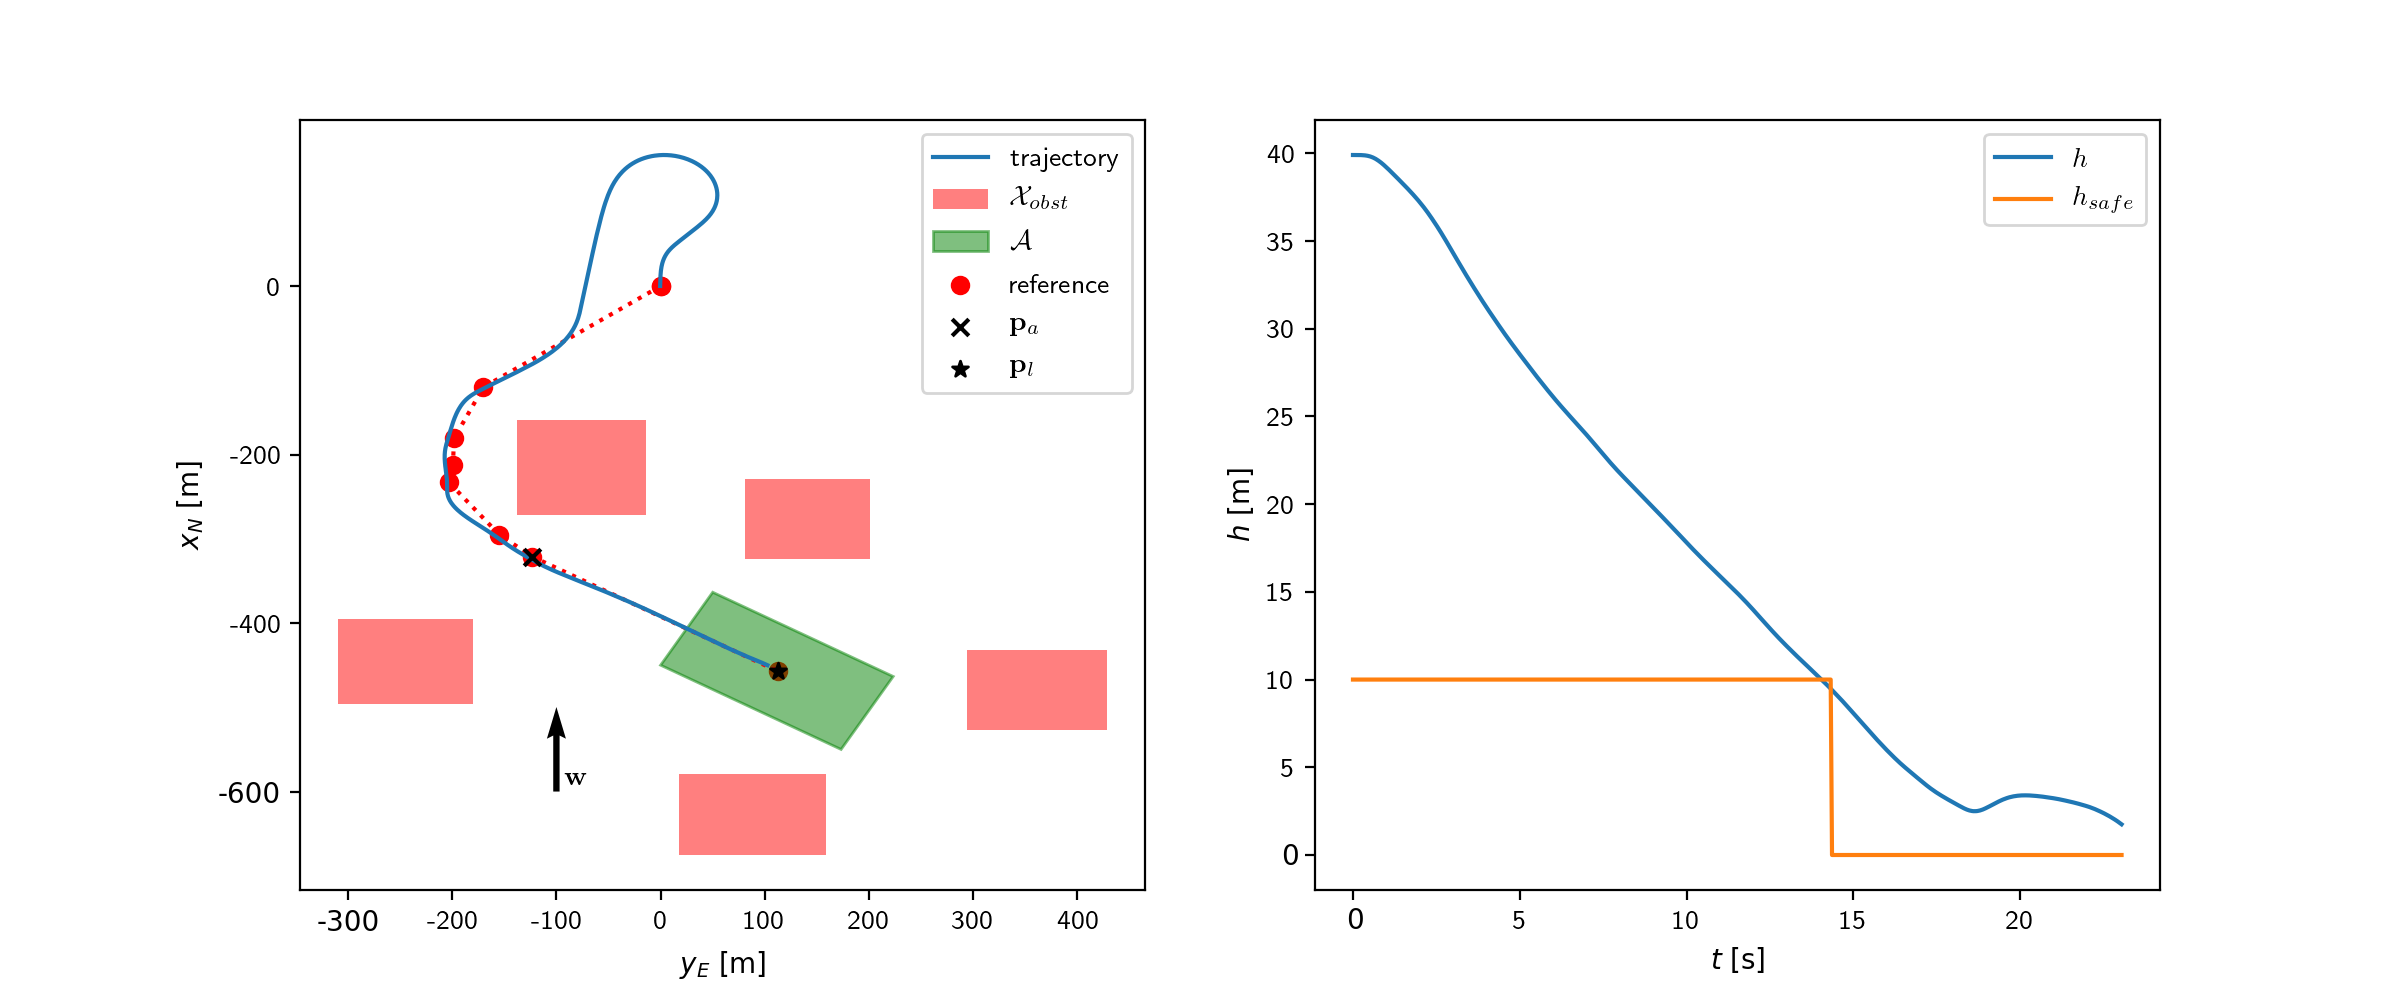
\includegraphics[width=.48\linewidth]{sol_0}
    }
    \subfloat[$\psi_w=90\degree$]{
        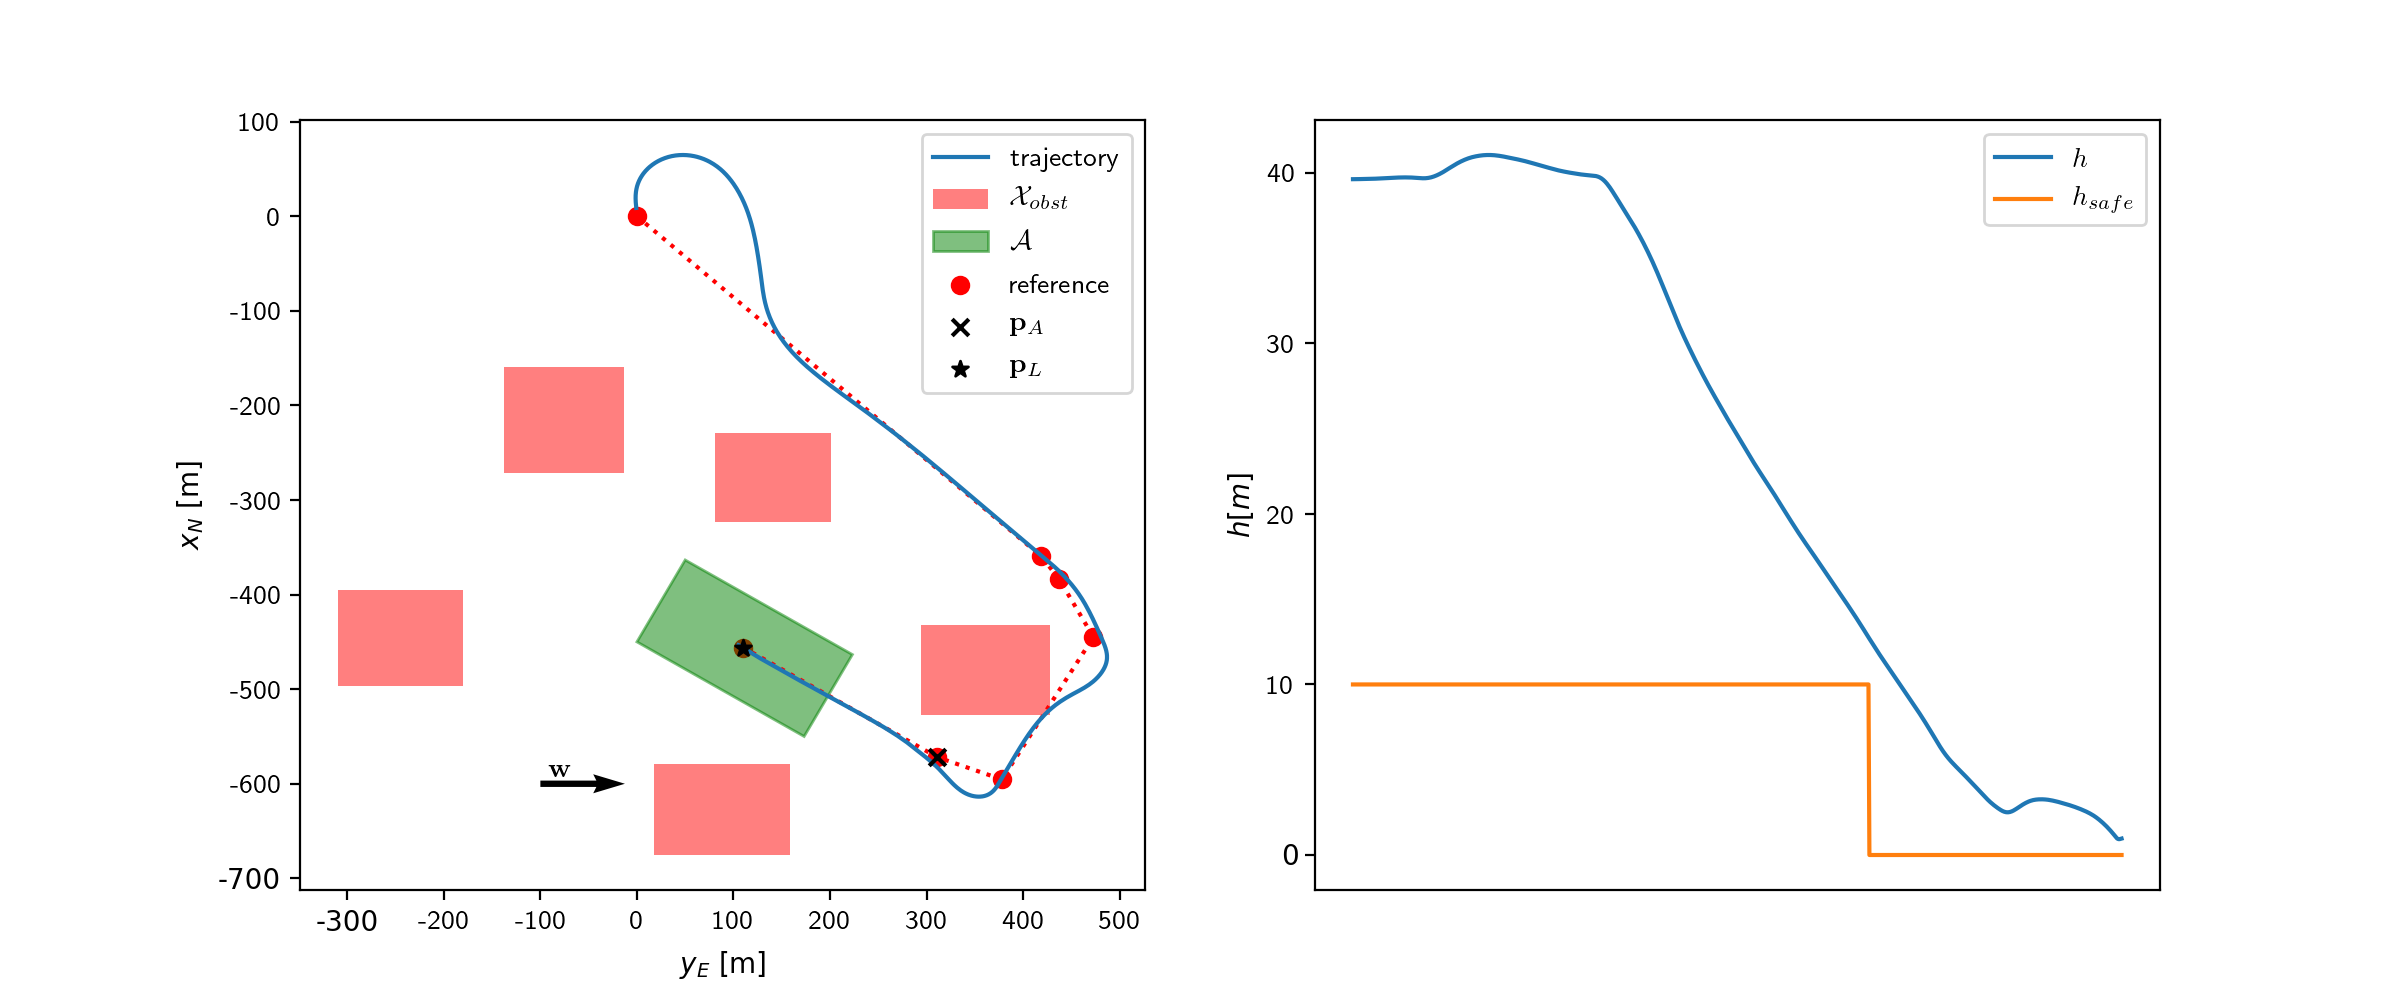
\includegraphics[width=.48\linewidth]{sol_90}
    }\\
    \subfloat[$\psi_w=180\degree$]{
        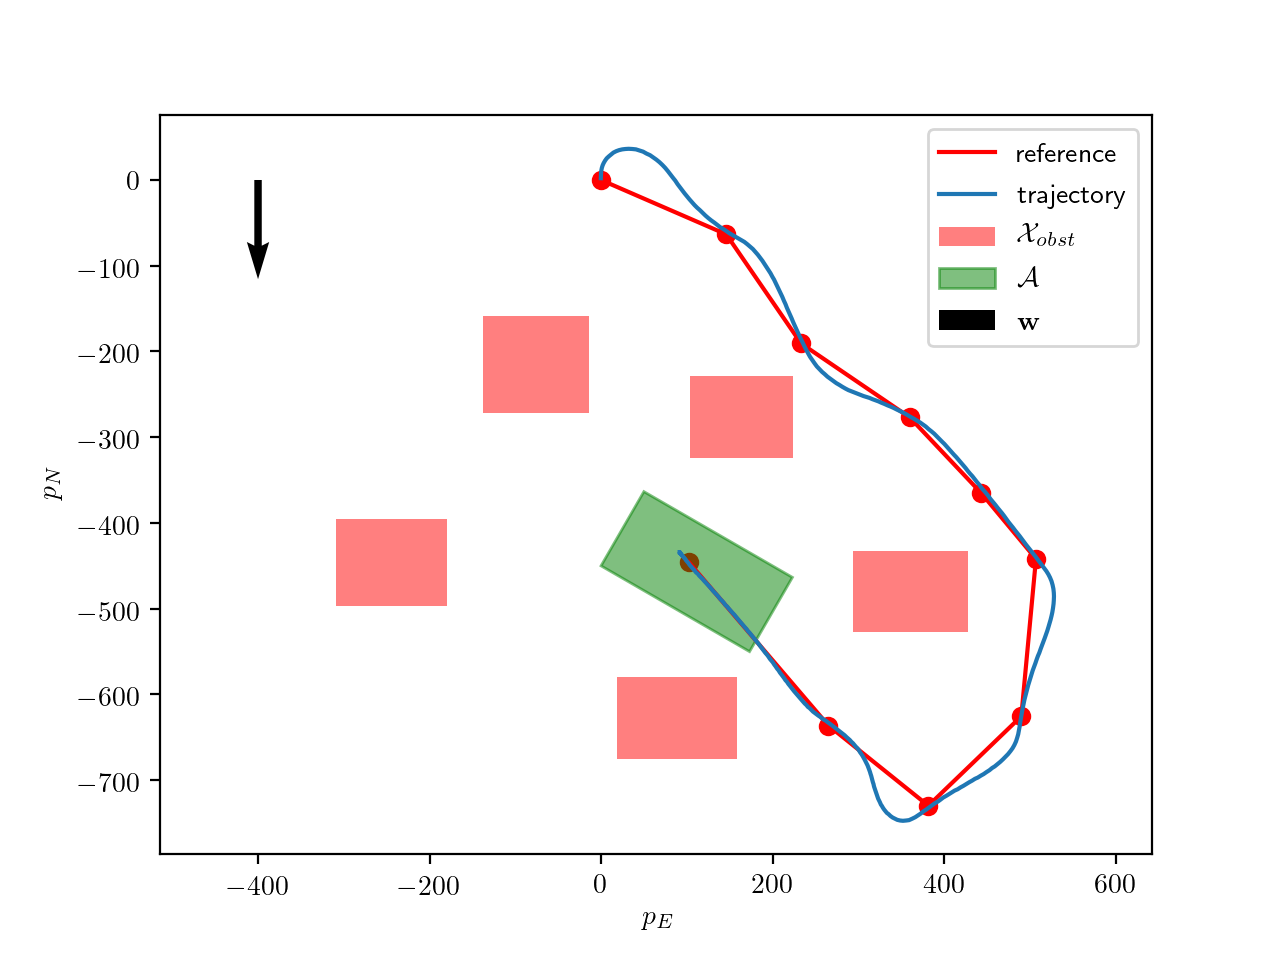
\includegraphics[width=.48\linewidth]{sol_180}
    }
    \subfloat[$\psi_w=270\degree$]{
        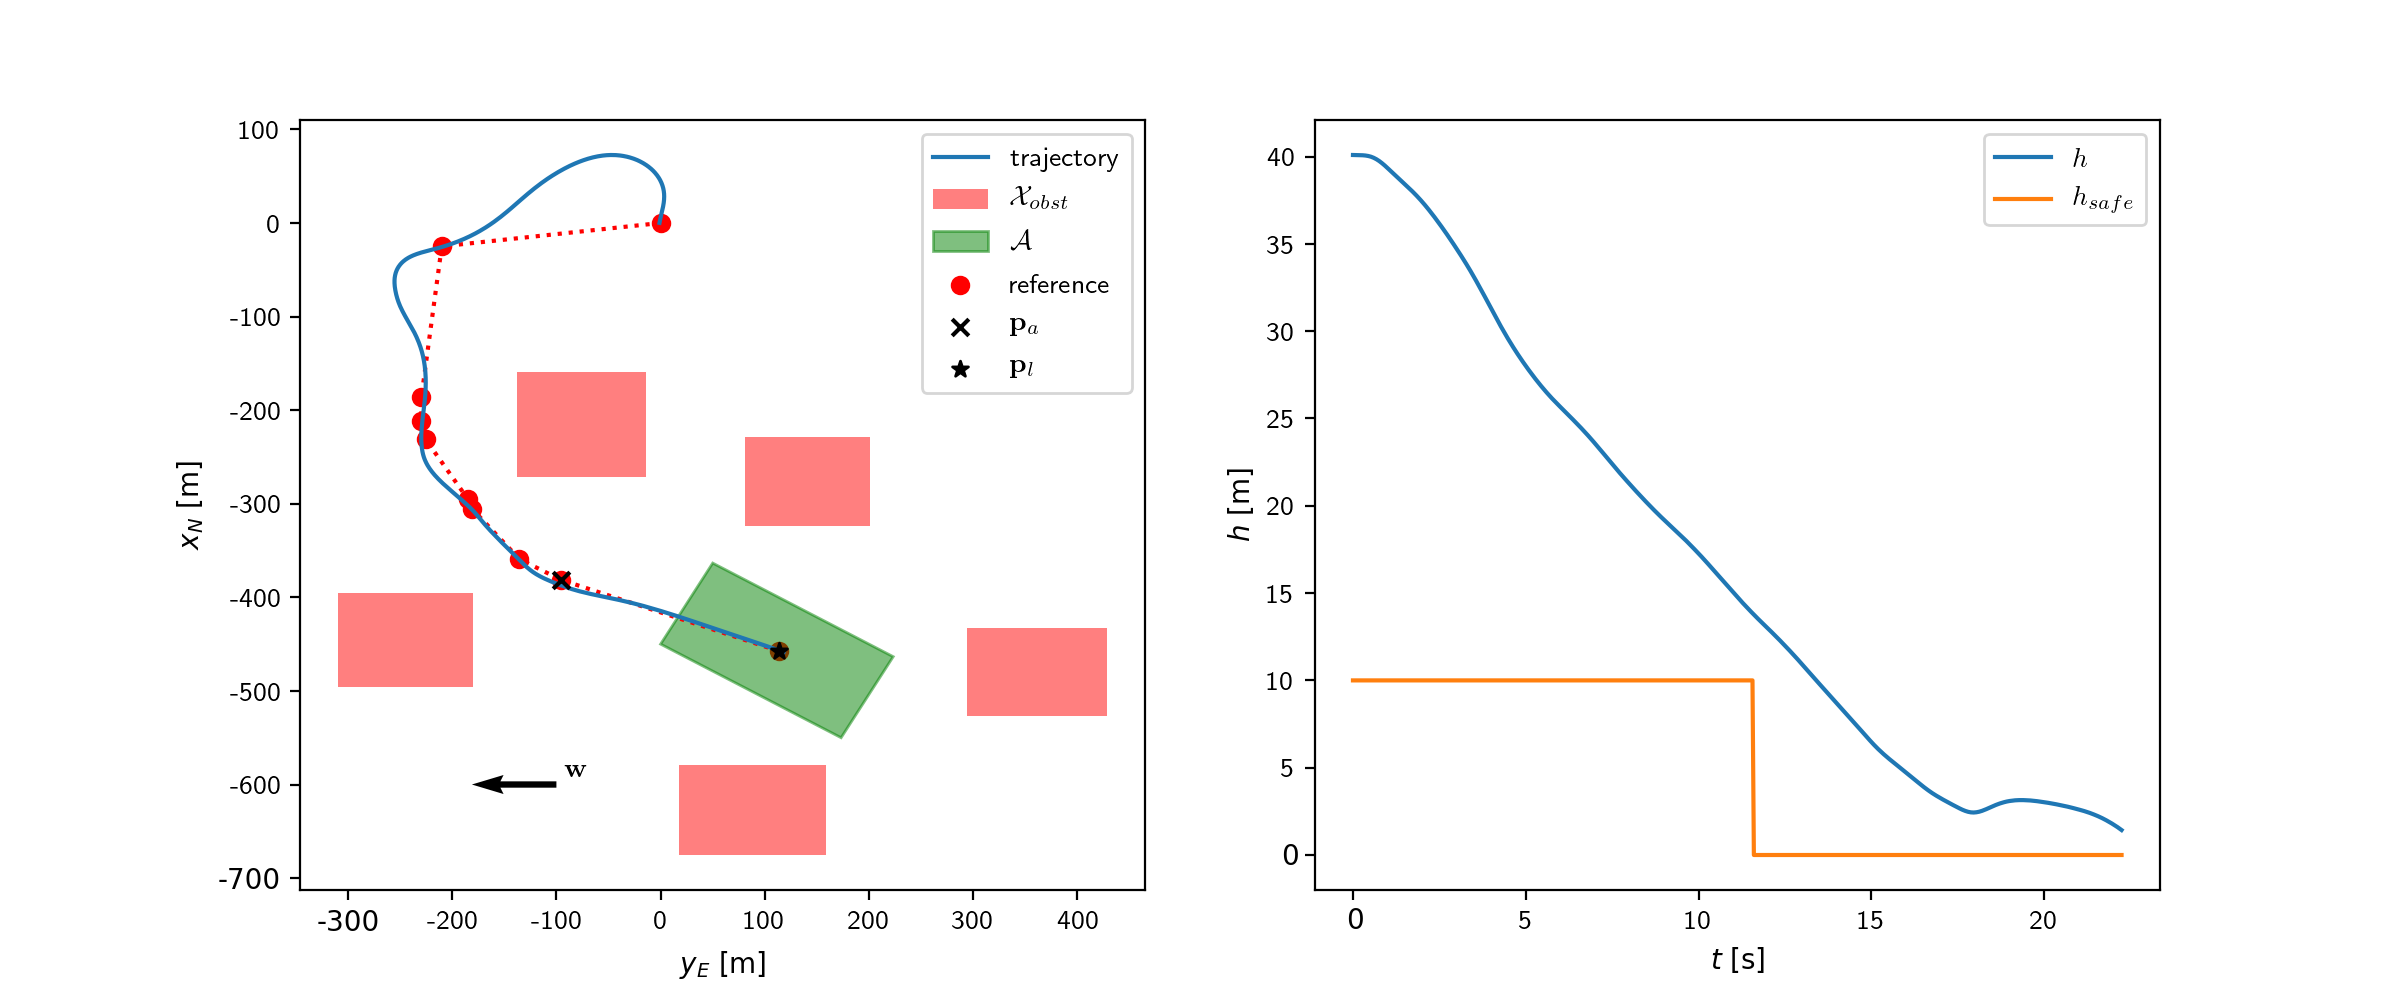
\includegraphics[width=.48\linewidth]{sol_270}
    }
    \caption{Resulting landing procedures for different wind directions, $W=5$ m/s}
    \label{fig:result}
\end{figure}

The calculated optimal landing parameters are summarized in Table \ref{tab:opt_land_param}. The distance $|R_a-R_b|$ corresponds to the total distance between the landing points,
and the distance $|R_c-R_c|$ corresponds to the distance from the landing to the center of $\mathcal{A}$.

\begin{table}
    \begin{center}
        \begin{tabular}{|c|c|c|c|c|}
            \hline
            $\psi_w$ & $\psi_L^*$ & $|R_a^*-R_b^*|$ & $|R_b^*-R_c|$\\
            \hline
            $0\degree$ & $230\degree$ & 209.8 m & 42.2 m \\
            \hline
            $90\degree$ & $250\degree$ & 173.4 m & 13.5 m \\
            \hline
            $180\degree$ & $320\degree$ & 195.5 m & 14.4 m  \\
            \hline
            $270\degree$ & $70\degree$ & 173.4 m & 13.5 m  \\
            \hline
        \end{tabular}
    \end{center}
    \caption{Optimal landing parameters}
    \label{tab:opt_land_param}
\end{table}